\documentclass[ignorenonframetext,]{beamer}
\setbeamertemplate{caption}[numbered]
\setbeamertemplate{caption label separator}{: }
\setbeamercolor{caption name}{fg=normal text.fg}
\beamertemplatenavigationsymbolsempty
\usepackage{lmodern}
\usepackage{amssymb,amsmath}
\usepackage{ifxetex,ifluatex}
\usepackage{fixltx2e} % provides \textsubscript
\ifnum 0\ifxetex 1\fi\ifluatex 1\fi=0 % if pdftex
\usepackage[T1]{fontenc}
\usepackage[utf8]{inputenc}
\else % if luatex or xelatex
\ifxetex
\usepackage{mathspec}
\else
\usepackage{fontspec}
\fi
\defaultfontfeatures{Ligatures=TeX,Scale=MatchLowercase}
\fi
\usetheme{gcat}
% use upquote if available, for straight quotes in verbatim environments
\IfFileExists{upquote.sty}{\usepackage{upquote}}{}
% use microtype if available
\IfFileExists{microtype.sty}{%
\usepackage{microtype}
\UseMicrotypeSet[protrusion]{basicmath} % disable protrusion for tt fonts
}{}
\newif\ifbibliography
\usepackage{longtable,booktabs}
\usepackage{caption}
% These lines are needed to make table captions work with longtable:
\makeatletter
\def\fnum@table{\tablename~\thetable}
\makeatother

% Prevent slide breaks in the middle of a paragraph:
\widowpenalties 1 10000
\raggedbottom

\AtBeginPart{
\let\insertpartnumber\relax
\let\partname\relax
\frame{\partpage}
}
\AtBeginSection{
\ifbibliography
\else
\let\insertsectionnumber\relax
\let\sectionname\relax
\frame{\sectionpage}
\fi
}
\AtBeginSubsection{
\let\insertsubsectionnumber\relax
\let\subsectionname\relax
\frame{\subsectionpage}
}

\setlength{\parindent}{0pt}
\setlength{\parskip}{6pt plus 2pt minus 1pt}
\setlength{\emergencystretch}{3em}  % prevent overfull lines
\providecommand{\tightlist}{%
\setlength{\itemsep}{0pt}\setlength{\parskip}{0pt}}
\setcounter{secnumdepth}{0}

\title{Regles d'associació de malalties i medicació a GCAT}
\author{Xavier Duran Albareda\\
GCAT Genomes for Life\\
Institut de Recerca Germans Trias i Pujol (IGTP)}
\date{29 de Novembre del 2016}

\begin{document}
\frame{\titlepage}

\begin{frame}{Codificació de les malalties}

\begin{block}{CIM-9-MC}

La CIM-9-MC és l'instrument de referència a Catalunya per codificar
malalties i procediments en l'àmbit hospitalari, en el de la salut
mental (tant d'internament com d'atenció ambulatòria) i en el dels
recursos sociosanitaris, i en alguns centres d'atenció primària, entre
d'altres.

\end{block}

\begin{block}{CIM-10-MC/PCS}

La CIM-10-MC/PCS serà el nou estàndard per a la codificació de malalties
i procediments a Catalunya i es preveu que entri en vigor a partir de
l'1 de gener de 2017.

\end{block}

\end{frame}

\begin{frame}{Codificació de les malalties}

\begin{block}{CIM-10-MC/PCS}

\begin{itemize}
\tightlist
\item
  es passa de 16.019 codis a 82.108
\item
  s'afegeix informació rellevant per a l'atenció ambulatòria
\item
  s'amplien els codis de lesions
\item
  la nova estructura permet l'expansió futura de la classificació
\end{itemize}

\begin{figure}[v]
  \mbox{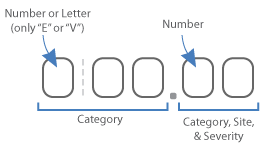
\includegraphics[height=.8in]{images/Training_icd9_example.png}}
  \mbox{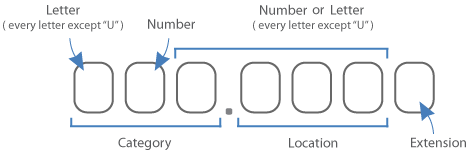
\includegraphics[height=.8in]{images/Training_icd10_conversionV2.png}}
  \caption{CIM-9-MC i CIM-10-MC/PCS}\label{fig:conversion}
\end{figure}

\end{block}

\end{frame}

\begin{frame}{Codificació de les malalties}

\begin{block}{CIM-9-MC a CIM-10-MC/PCS. Exemple (diabetis)}

\begin{longtable}[]{@{}lll@{}}
\caption{Codificació CIM-9-MC i CIM-10-MC/PCS de la
Diabetis}\tabularnewline
\toprule
Estàndard & Codificació & Descripció\tabularnewline
\midrule
\endfirsthead
\toprule
Estàndard & Codificació & Descripció\tabularnewline
\midrule
\endhead
CIM-9-MC & 25000 & Diabetis mellitus sense menció\tabularnewline
& & de complicació, tipus II\tabularnewline
& & o tipus no especificat,\tabularnewline
& & no esmentada com a incontrolada\tabularnewline
CIM-10-MC/PCS & E119 & Diabetis mellitus de tipus 2\tabularnewline
\bottomrule
\end{longtable}

\end{block}

\end{frame}

\begin{frame}{Codificació de les malalties}

\begin{block}{Codificació de les malalties autoreportades a CIM-9-MC}

\begin{table}[ht]
\begin{flushleft}
\scalebox{0.4}{
\begin{tabular}{lrll}
  \hline
Text & Freqüència & Codi & Descripció \\ 
  \hline
HIPERCOLESTEROLEMIA & 2523 & 2720 & Hipercolesterolèmia pura \\ 
  ALERGIA & 2211 & 9953 & Al·lèrgia no especificada \\ 
  HTA & 2059 & 401 & Hipertensió essencial \\ 
  MIGRANA & 1171 & 346 & Migranya \\ 
  RINITIS & 1008 & 4720 & Rinitis crònica \\ 
  DEPRESION & 910 & 311 & Trastorn depressiu no classificat a cap altre lloc \\ 
  ASMA & 701 & 493 & Asma \\ 
  ECZEMA & 610 & 692 & Dermatitis de contacte i altres èczemes \\ 
  HELICOBACTER & 578 & 04186 & Infecció per Helicobacter pylori [H. pylori] en afeccions classificades en un altre lloc i de localització no especificada \\ 
  POLIPOS & 518 & 5690 & Pòlip anal i rectal \\ 
  PSORIASIS & 487 & 696 & Psoriasi i trastorns semblants \\ 
  DIABETES & 461 & 250 & Diabetis mellitus \\ 
  OSTEOPOROSIS & 457 & 7330 & Osteoporosi \\ 
  ARTRITIS & 397 & 714 & Artritis reumatoide i altres poliartropaties inflamatòries \\ 
  HIPOTIROIDISMO & 306 & 2449 & Hipotiroïdisme no especificat \\ 
  CANCER & 289 & 1991 & Altres neoplàsies malignes de localització no especificada \\ 
  ANSIEDAD & 280 & 30000 & Estat d'ansietat no especificat \\ 
  INSOMNIO & 254 & 78050 & Trastorn del son no especificat \\ 
  TIROIDES & 189 & 226 & Neoplàsia benigna de glàndules tiroides \\ 
  DOLOR & 165 & 338 & Dolor no classificat a cap altre lloc \\ 
   \hline
\end{tabular}
}
\caption{Codificació manual de les malalties} 
\end{flushleft}
\end{table}

\end{block}

\end{frame}

\begin{frame}{Codificació de les malalties}

\begin{block}{Codificació de les malalties autoreportades a CIM-9-MC}

\begin{table}[ht]
\begin{flushleft}
\scalebox{0.4}{
\begin{tabular}{lrll}
  \hline
Text & Freqüència & Codi & Descripció \\ 
  \hline
HIPERCOLESTEROLEMIA & 2523 & 272 & Trastorns del metabolisme dels lípids \\ 
  ALERGIA & 2211 & 995 & Determinades reaccions adverses no classificades a cap altre lloc \\ 
  HTA & 2059 & 401 & Hipertensió essencial \\ 
  MIGRANA & 1171 & 346 & Migranya \\ 
  RINITIS & 1008 & 472 & Faringitis i rinofaringitis cròniques \\ 
  DEPRESION & 910 & 311 & Trastorn depressiu no classificat a cap altre lloc \\ 
  ASMA & 701 & 493 & Asma \\ 
  ECZEMA & 610 & 692 & Dermatitis de contacte i altres èczemes \\ 
  HELICOBACTER & 578 & 041 & Infeccions bacterianes en afeccions classificades en un altre lloc i de localització no especificada \\ 
  POLIPOS & 518 & 569 & Altres trastorns d'intestí \\ 
  PSORIASIS & 487 & 696 & Psoriasi i trastorns semblants \\ 
  DIABETES & 461 & 250 & Diabetis mellitus \\ 
  OSTEOPOROSIS & 457 & 733 & Altres trastorns de l'os i el cartílag \\ 
  ARTRITIS & 397 & 714 & Artritis reumatoide i altres poliartropaties inflamatòries \\ 
  HIPOTIROIDISMO & 306 & 244 & Hipotiroïdisme adquirit \\ 
  CANCER & 289 & 199 & Neoplàsia maligna de localització no especificada \\ 
  ANSIEDAD & 280 & 300 & Trastorns d'ansietat, dissociatiu i somatomorf \\ 
  INSOMNIO & 254 & 780 & Símptomes generals \\ 
  TIROIDES & 189 & 226 & Neoplàsia benigna de glàndules tiroides \\ 
  DOLOR & 165 & 338 & Dolor no classificat a cap altre lloc \\ 
   \hline
\end{tabular}
}
\caption{Codificació manual de les malalties} 
\end{flushleft}
\end{table}

\end{block}

\end{frame}

\begin{frame}{Codificació de la medicació}

\begin{block}{ATC}

El codi ATC o Sistema de Classificació Química Anatomicoterapèutica és
un índex de substàncies farmacològiques i medicaments, organitzats
segons grups terapèutics.

El codi arreplega el sistema o òrgan sobre el qual actua, l'efecte
farmacològic, les indicacions terapèutiques i l'estructura química del
fàrmac.

\begin{longtable}[]{@{}lll@{}}
\caption{Codificació ATC de la Metformina}\tabularnewline
\toprule
Nivell ATC & Codi ATC & Descripció\tabularnewline
\midrule
\endfirsthead
\toprule
Nivell ATC & Codi ATC & Descripció\tabularnewline
\midrule
\endhead
Grup anatòmic & A & Sistema digestiu i metabolisme\tabularnewline
Grup terapèutic & A10 & Fàrmacs usats en diabetis\tabularnewline
Subgrup farmacològic & A10B & Fàrmacs hipoglucemiants
orals\tabularnewline
Subgrup químic & A10B A & Biguanides\tabularnewline
Substància química & A10B A02 & Metformina\tabularnewline
\bottomrule
\end{longtable}

\end{block}

\end{frame}

\begin{frame}{Codificació de la medicació}

\begin{block}{Medicaments autoreportats al GCAT}

\begin{longtable}[]{@{}rl@{}}
\caption{Nombre i codificació de medicaments reportats}\tabularnewline
\toprule
\# Medicaments & Codificació\tabularnewline
\midrule
\endfirsthead
\toprule
\# Medicaments & Codificació\tabularnewline
\midrule
\endhead
14961 & codificats\tabularnewline
2406 & text lliure\tabularnewline
\bottomrule
\end{longtable}

Com podem transformar \emph{automàticament} els medicaments reportats en
text lliure?

\end{block}

\end{frame}

\begin{frame}{Codificació de la medicació}

\begin{block}{Medicaments autoreportats al GCAT}

Tranquimazin Retard 0.25 mg

\begin{itemize}
\tightlist
\item
  Convertir text a majúscules
\item
  Eliminar informació de dosatge
\item
  Eliminar puntuació
\item
  Buscar el terme més semblant al diccionari (distància de Levenshtein)
\end{itemize}

N05BA TRANKIMAZIN RETARD

\end{block}

\end{frame}

\begin{frame}{Codificació de la medicació}

\begin{block}{Conversió automàtica de text lliure. Resultats}

\begin{table}[ht]
\centering
\scalebox{0.4}{
\begin{tabular}{lllll}
  \hline
Text & Codi 90\% & Nom 90\% & Codi 80\% & Nom 80\% \\ 
  \hline
tansolosina &  &  & G04CA & TAMSULOSINA \\ 
  Blecometasona &  &  & R02AA & BUCOMETASANA \\ 
  metformina & A10BA & METFORMINA & A10BA & METFORMINA \\ 
  metformina & A10BA & METFORMINA & A10BA & METFORMINA \\ 
  METMORFINA 850 &  &  & N02AA & MORFINA \\ 
  JANUVIA & A10BH & JANUVIA & A10BH & JANUVIA \\ 
  metformina & A10BA & METFORMINA & A10BA & METFORMINA \\ 
  metformina & A10BA & METFORMINA & A10BA & METFORMINA \\ 
  Meformina & A10BA & METFORMINA & A10BA & METFORMINA \\ 
  Glicacida &  &  & A10BB & GLICLAZIDA \\ 
  METAFORMINA 850 & A10BA & METFORMINA & A10BA & METFORMINA \\ 
  MEFORMINA & A10BA & METFORMINA & A10BA & METFORMINA \\ 
  Metformina & A10BA & METFORMINA & A10BA & METFORMINA \\ 
  Meformina 850 mg & A10BA & METFORMINA & A10BA & METFORMINA \\ 
  novornom &  &  & A10BX & NOVONORM \\ 
  Metformina & A10BA & METFORMINA & A10BA & METFORMINA \\ 
  insulina &  &  & D01BA & SULVINA \\ 
  janumet & A10BD & JANUMET & A10BD & JANUMET \\ 
  EFICIB & A10BD & EFFICIB & A10BD & EFFICIB \\ 
  jardinet &  &  & J01CA & ARDINE \\ 
   \hline
\end{tabular}
}
\caption{Correcció automàtica de medicaments} 
\end{table}

\end{block}

\end{frame}

\begin{frame}{Codificació de la medicació}

\begin{block}{Conversió automàtica de text lliure. Resultats}

2406 medicaments no codificats

\begin{longtable}[]{@{}rrl@{}}
\caption{Conversió automàtica de text lliure a ATC}\tabularnewline
\toprule
Semblança (\%) & Cobertura & Descripció\tabularnewline
\midrule
\endfirsthead
\toprule
Semblança (\%) & Cobertura & Descripció\tabularnewline
\midrule
\endhead
90\% & 735/2406 & Fiable\tabularnewline
80\% & 1206/2406 & A vegades s'equivoca\tabularnewline
70\% & 1825/2406 & Massa errors\tabularnewline
\bottomrule
\end{longtable}

\end{block}

\end{frame}

\begin{frame}{Regles d'associació}

\begin{block}{Definició}

Les regles d'associació troben patrons freqüents, associacions o
correlacions entre conjunts d'ítems en bases de dades de transaccions.
Donat un conjunt de transaccions, trobarem regles que prediguin
l'ocurrència d'un ítem basat en la presència d'altres ítems en la
transacció.

\begin{longtable}[]{@{}ll@{}}
\toprule
Transacció & Items\tabularnewline
\midrule
\endhead
=E0025********21 & A10 Drugs used in diabetes\tabularnewline
=E0025********21 & 250 Diabetis mellitus\tabularnewline
=E0025********21 & C07 Beta blocking agents\tabularnewline
=E0025********21 & SEXE=1\tabularnewline
=E0025********21 & EDAT={[}55,65{]}\tabularnewline
=E0025********21 & WHR={[}0.909,1.226{]}\tabularnewline
\bottomrule
\end{longtable}

\end{block}

\end{frame}

\begin{frame}{Regles d'associació}

A10 Drugs used in diabetes \(\Rightarrow\) 250 Diabetis mellitus
{[}support=2\%, confidence=93\%, lift=26.73, \(\chi^2\)=6414.32{]}

\begin{block}{Indicadors}

\(support(A \Rightarrow B) = P(A \cup B)\)

\(confidence(A \Rightarrow B) = P(B|A) = \frac{P(A \cup B)}{P(A)}\)

\(lift(A \Rightarrow B) = confidence(A \Rightarrow B)/P(B) = \frac{P(A \cup B)}{P(A)P(B)}\)

\(\chi^2(A \Rightarrow B) = n\frac{P(A)P(B)}{(1-P(A))(1-P(B))}\)

\end{block}

\end{frame}

\begin{frame}{Regles d'associació}

\begin{block}{Resultats}

\begin{table}[ht]
\centering
\scalebox{0.3}{
\begin{tabular}{llrrrr}
  \hline
lhs & rhs & support & confidence & lift & chiSquare \\ 
  \hline
A10 Drugs used in diabetes & X250 Diabetis mellitus & 1.86 & 93.07 & 26.73 & 6675.95 \\ 
  C09 Agents acting on the renin.angiotensin system & X401 Hipertensio essencial & 8.21 & 94.86 & 6.26 & 6414.32 \\ 
  R03 Anti.asthmatics & X493 Asma & 2.17 & 82.50 & 15.65 & 4416.39 \\ 
  X401 Hipertensio essencial,A10 Drugs used in diabetes & X250 Diabetis mellitus & 0.99 & 95.07 & 27.30 & 3581.16 \\ 
  X272 Trastorns del metabolisme dels lipids,A10 Drugs used in diabetes & X250 Diabetis mellitus & 0.87 & 95.97 & 27.56 & 3184.56 \\ 
  X401 Hipertensio essencial,S01 Ophthalmologicals & X365 Glaucoma & 0.15 & 66.67 & 154.78 & 3075.68 \\ 
  C10 Lipid modifying agents & X272 Trastorns del metabolisme dels lipids & 6.11 & 79.87 & 4.56 & 3052.40 \\ 
  X995 Determinades reaccions adverses no classificades a cap altre lloc,R03 Anti.asthmatics & X493 Asma & 1.47 & 84.10 & 15.96 & 3027.31 \\ 
  A10 Drugs used in diabetes,C10 Lipid modifying agents & X250 Diabetis mellitus & 0.77 & 93.75 & 26.92 & 2737.67 \\ 
  A10 Drugs used in diabetes,C09 Agents acting on the renin.angiotensin system & X250 Diabetis mellitus & 0.69 & 92.23 & 26.49 & 2432.15 \\ 
  A12 Mineral supplements & X733 Altres trastorns de l.os i el cartilag & 0.94 & 65.15 & 19.07 & 2320.38 \\ 
  X272 Trastorns del metabolisme dels lipids,C09 Agents acting on the renin.angiotensin system & X401 Hipertensio essencial & 2.81 & 96.73 & 6.38 & 2121.50 \\ 
  M05 Drugs for treatment of bone diseases & X733 Altres trastorns de l.os i el cartilag & 0.55 & 88.37 & 25.87 & 1892.89 \\ 
  R06 Antihistamines for systemic use & X995 Determinades reaccions adverses no classificades a cap altre lloc & 3.23 & 85.69 & 5.19 & 1863.71 \\ 
  X472 Faringitis i rinofaringitis croniques,R03 Anti.asthmatics & X493 Asma & 0.76 & 88.89 & 16.86 & 1652.52 \\ 
  L02 Endocrine therapy & X199 Neoplasia maligna de localitzacio no especificada & 0.24 & 91.67 & 42.56 & 1372.49 \\ 
  C09 Agents acting on the renin.angiotensin system,C10 Lipid modifying agents & X401 Hipertensio essencial & 1.89 & 92.17 & 6.08 & 1323.33 \\ 
  R01 Nasal preparations & X472 Faringitis i rinofaringitis croniques & 1.09 & 73.04 & 9.60 & 1261.48 \\ 
  X995 Determinades reaccions adverses no classificades a cap altre lloc,A10 Drugs used in diabetes & X250 Diabetis mellitus & 0.34 & 95.83 & 27.52 & 1222.31 \\ 
  X401 Hipertensio essencial,C10 Lipid modifying agents & X272 Trastorns del metabolisme dels lipids & 2.29 & 82.80 & 4.73 & 1146.44 \\ 
  A12 Mineral supplements,M05 Drugs for treatment of bone diseases & X733 Altres trastorns de l.os i el cartilag & 0.28 & 95.00 & 27.81 & 1019.70 \\ 
  R03 Anti.asthmatics,R06 Antihistamines for systemic use & X493 Asma & 0.51 & 81.40 & 15.44 & 1004.43 \\ 
  C03 Diuretics & X401 Hipertensio essencial & 1.58 & 84.71 & 5.59 & 977.48 \\ 
  X995 Determinades reaccions adverses no classificades a cap altre lloc,C09 Agents acting on the renin.angiotensin system & X401 Hipertensio essencial & 1.27 & 97.21 & 6.41 & 949.60 \\ 
  X995 Determinades reaccions adverses no classificades a cap altre lloc,R01 Nasal preparations & X472 Faringitis i rinofaringitis croniques & 0.77 & 72.60 & 9.54 & 887.01 \\ 
  D07 Corticosteroids dermatological preparations & X692 Dermatitis de contacte i altres eczemes & 0.48 & 62.86 & 13.69 & 819.92 \\ 
  D05 Antipsoriatics & X696 Psoriasi i trastorns semblants & 0.24 & 94.29 & 25.73 & 816.22 \\ 
  C09 Agents acting on the renin.angiotensin system,C10 Lipid modifying agents & X272 Trastorns del metabolisme dels lipids & 1.63 & 79.36 & 4.53 & 759.15 \\ 
  X311 Trastorn depressiu no classificat a cap altre lloc,A10 Drugs used in diabetes & X250 Diabetis mellitus & 0.20 & 96.43 & 27.69 & 721.18 \\ 
  C07 Beta blocking agents & X401 Hipertensio essencial & 1.44 & 73.23 & 4.83 & 719.79 \\ 
  X272 Trastorns del metabolisme dels lipids,R03 Anti.asthmatics & X493 Asma & 0.39 & 76.81 & 14.57 & 710.86 \\ 
  X472 Faringitis i rinofaringitis croniques,R06 Antihistamines for systemic use & X995 Determinades reaccions adverses no classificades a cap altre lloc & 1.33 & 82.35 & 4.98 & 705.87 \\ 
  A10 Drugs used in diabetes,N06 Psychoanaleptics & X250 Diabetis mellitus & 0.21 & 87.88 & 25.24 & 701.04 \\ 
  A10 Drugs used in diabetes,B01 Antithrombotic agents & X250 Diabetis mellitus & 0.18 & 100.00 & 28.72 & 694.19 \\ 
  A12 Mineral supplements,G03 Sex hormones and modulators of the genital system & X733 Altres trastorns de l.os i el cartilag & 0.25 & 72.34 & 21.17 & 678.95 \\ 
  R01 Nasal preparations,R06 Antihistamines for systemic use & X472 Faringitis i rinofaringitis croniques & 0.50 & 83.13 & 10.93 & 677.73 \\ 
  C08 Calcium channel blockers & X401 Hipertensio essencial & 0.95 & 93.53 & 6.17 & 670.73 \\ 
  R01 Nasal preparations,R03 Anti.asthmatics & X493 Asma & 0.31 & 87.76 & 16.65 & 670.09 \\ 
  R03 Anti.asthmatics & X995 Determinades reaccions adverses no classificades a cap altre lloc & 1.74 & 66.39 & 4.02 & 666.67 \\ 
  G03 Sex hormones and modulators of the genital system,R03 Anti.asthmatics & X493 Asma & 0.34 & 82.14 & 15.58 & 665.49 \\ 
   \hline
\end{tabular}
}
\caption{Relacions entre malalties i medicaments inferides} 
\end{table}

\end{block}

\end{frame}

\begin{frame}{Regles d'associació}

\begin{block}{Aplicació Shiny}

\begin{figure}[v]
  \mbox{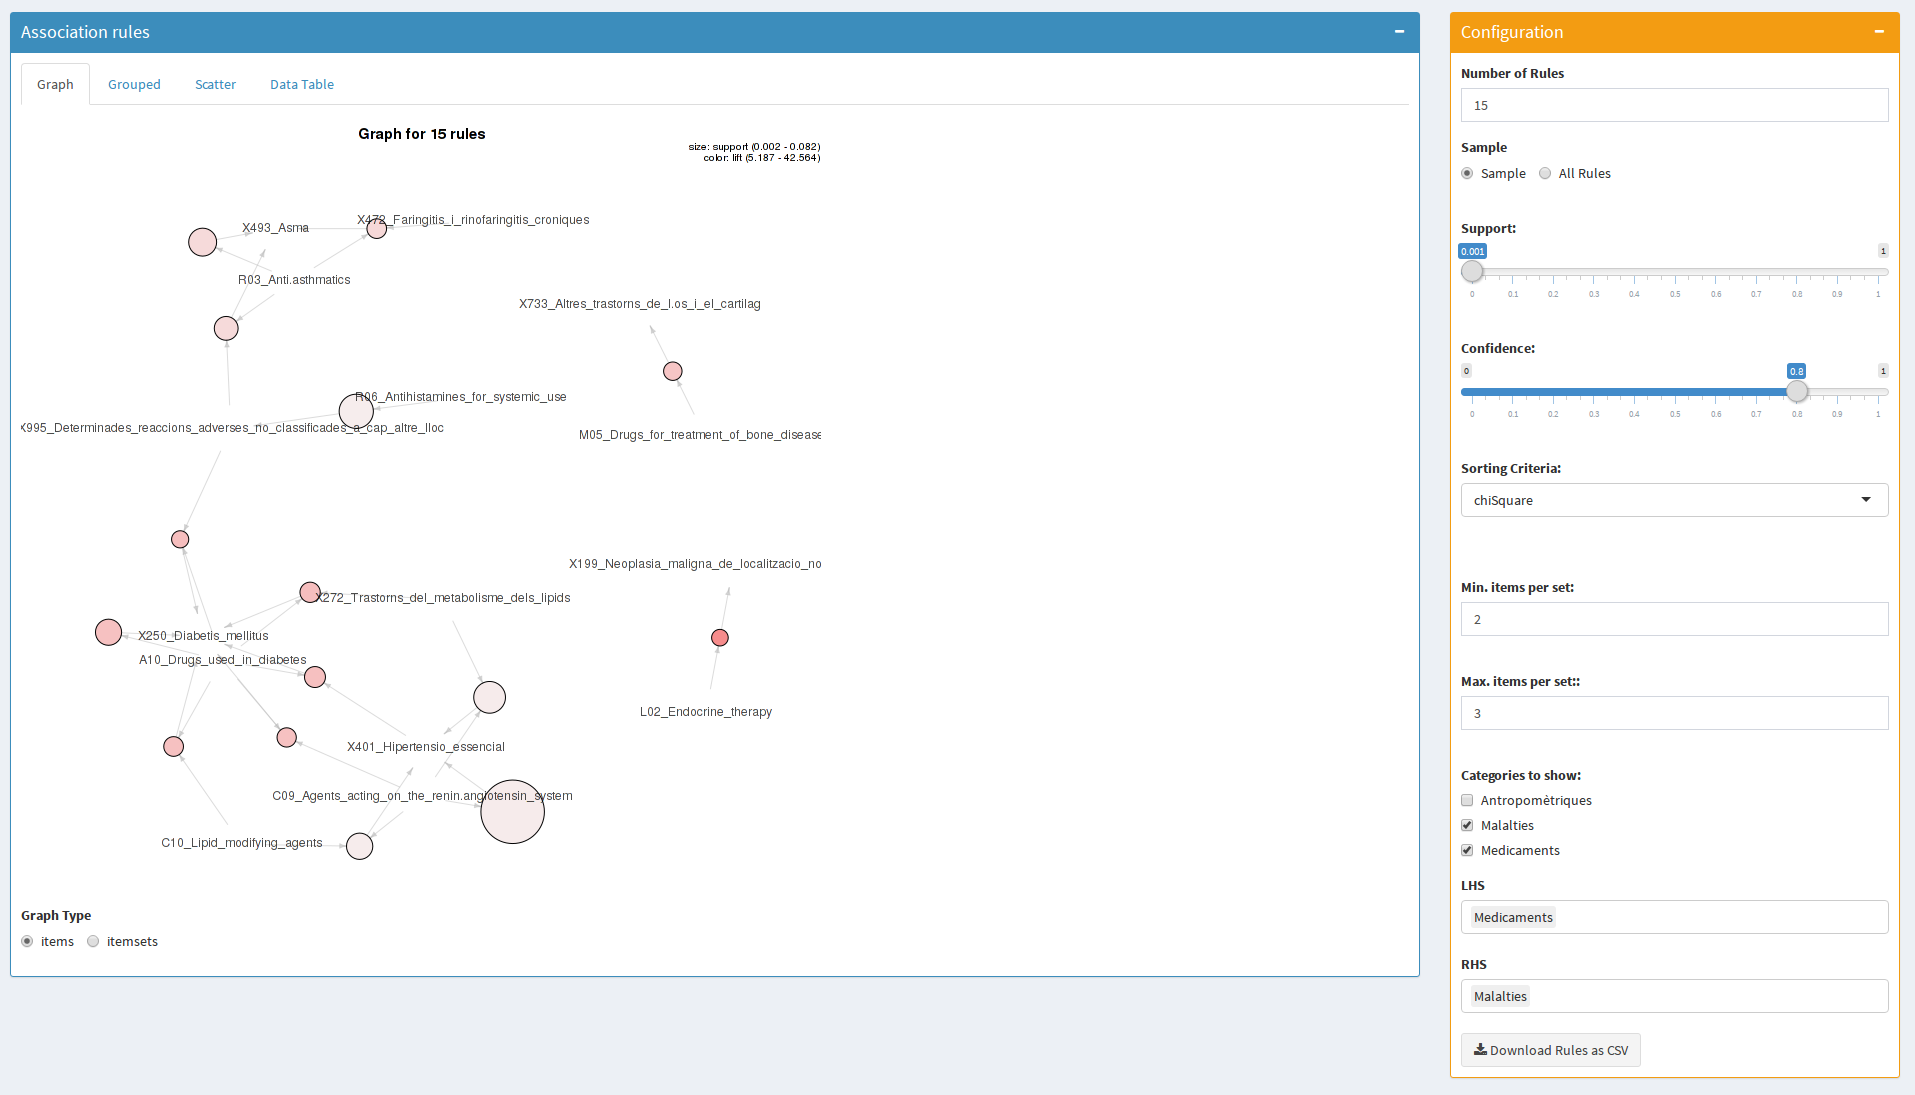
\includegraphics[height=2in]{images/medsnrules.png}}
  \caption{https://xdurana.shinyapps.io/rules/}\label{fig:medsnrules}
\end{figure}

\end{block}

\end{frame}

\end{document}
